\chapter{Introduction}
\section{Question de recherche}

A partir de données sur le climat, la qualité du sol et les pratiques culturales, est-il possible d’expliquer et de prédire les différents traits de la qualité en bouche des cafés du département de Risaralda ?



\section{Contexte du projet}
Le sujet de ce Travail de Bachelor a été proposé par le « \textit{Centro Internacional de Agricultura Tropical }» (CIAT) qui travaille dans le but d’améliorer la productivité et la gestion de l’agriculture en zone tropicale, et dont les bureaux se trouvent à Cali, en Colombie.\\

À 200 kilomètres de Cali, le comité des caféiculteurs de Risaralda souhaite pouvoir expliquer les différents traits de la qualité en bouche des cafés produits dans les différents secteurs de leur département. La filière café colombienne est en effet en concurrence avec d’autres pays exportateurs sur le marché international, et un des avantages comparatifs de la Colombie est que ses terroirs produisent des cafés de qualité et de caractères affirmés. Il est donc stratégique pour la fédération des caféiculteurs de Colombie d'être en mesure de faire valoir ces spécificités pour aller chercher la valeur ajoutée associée aux produits démarqués du lot.\\


Ce projet a pour but de trouver des méthodes de modélisation afin d’identifier les caractéristiques du café spécifiques à chaque secteur de la région en se basant sur des analyses gustatives, des données climatiques et géographiques, et d’autres données de pratiques culturales.\\


Dans un premier temps, l’objectif est de catégoriser les cafés en tentant de trouver des tendances gustatives par rapport aux conditions de culture. Dans un second temps, il faudra pouvoir prédire la qualité en bouche des cafés par rapport aux conditions environnementales.\\


Le but de cette collaboration sur le long terme est de permettre au département de Risaralda de mettre en valeur la diversité de ses cafés, principalement à des fins de promotion auprès des acheteurs. \\


\section{Contexte des données}
\paragraph{Les données gustatives}sont très relatives aux sens et à la perception de chaque goutteur. Cependant, la SCAA, \textit{Speciality Coffee Association of America}, dispose d’un système de notation basé sur des hypothèses communautaires reconnues ce qui permet d’avoir une certaine régularité dans les données de dégustations. Les cafés sont notés sur 100 points répartis sur plusieurs critères: parfum/arôme, saveur, arrière-goût, acidité, corps, équilibre, douceur, clean-cup (absence de défauts marqués), uniformité et évaluation personnelle du testeur.  Chacun de ces critères est noté sur 10 mais aussi par des termes qualitatifs. Par exemple, la saveur, c’est-à-dire la combinaison de l’odeur et du goût, la première impression qu’on a en goûtant le café, peut être notée 7/10 et “Caramel”. 

\paragraph{Les données climatiques}comprennent les températures maximales, minimales et moyennes, la variation de température pendant la journée (DTR) et les quantités de précipitations. Les moyennes de ces mesures ont été calculée pour chaque mois et extrapolées sur une grande partie du territoire, permettant ainsi d’accéder aux mesures selon l’emplacement désiré à environ 500 mètres près. 

\paragraph{Les données de qualité de sol}sont subdivisées en profils. Chaque profil est séparé en une ou plusieurs couches d’une certaine profondeur dont sont renseignées les caractéristiques comme le pH, la gravimétrie ou encore le taux de matière organique. 

%TODO
\paragraph{Le système SICA}, pour \textit{Sistema de Información Cafetera}, 


\chapter{Processus de modélisation}
\section{Régression}
Les différents objectifs de ce projet étant d'un côté de classifier les différents cafés en leur trouvant des caractéristiques distinctes et de l'autre de prédire dans quelle catégorie un nouveau café se trouverait, différentes méthodes d'analyse seront utilisées. Afin d'analyser les relations entre les différentes variables, différentes méthodes de régression seront utilisées. 

% https://georgemdallas.wordpress.com/2013/10/30/principal-component-analysis-4-dummies-eigenvectors-eigenvalues-and-dimension-reduction/

% http://mengnote.blogspot.ch/2013/05/an-intuitive-explanation-of-pca.html


\subsection{Principal Component Analysis (PCA)}
La PCA, pour Analyse en Composante Principale en français, est une méthode qui consiste à transformer un set de variables corrélées en nouvelles variables dé-corrélées les unes des autres. Ces nouvelles variables sont appelées composantes principales et permettent de rendre l'information moins redondante. Pour faire plus simple, l'utilité de la Composante Principale est de réduire le nombre de variables tout en gardant un maximum d'information. 


\begin{figure}[]
	\caption{\label{PCAdefinition} Description de l'Analyse en Composante Principale }
	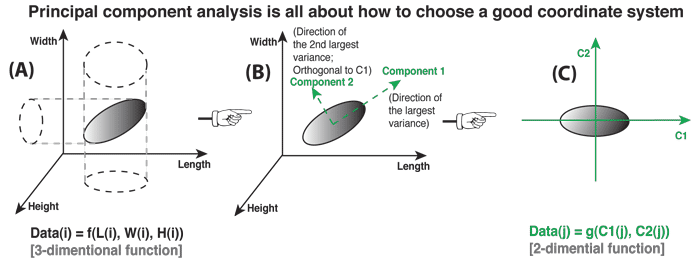
\includegraphics[scale=1]{PCA_1}
\end{figure}

